\documentclass[tikz,border=5pt]{standalone}
\usepackage{fontspec}
\setmainfont{Times New Roman}
\usepackage{unicode-math}
\setmathfont{Cambria Math}
\usetikzlibrary{shapes.geometric,positioning,fit,backgrounds,arrows.meta,calc}

\begin{document}
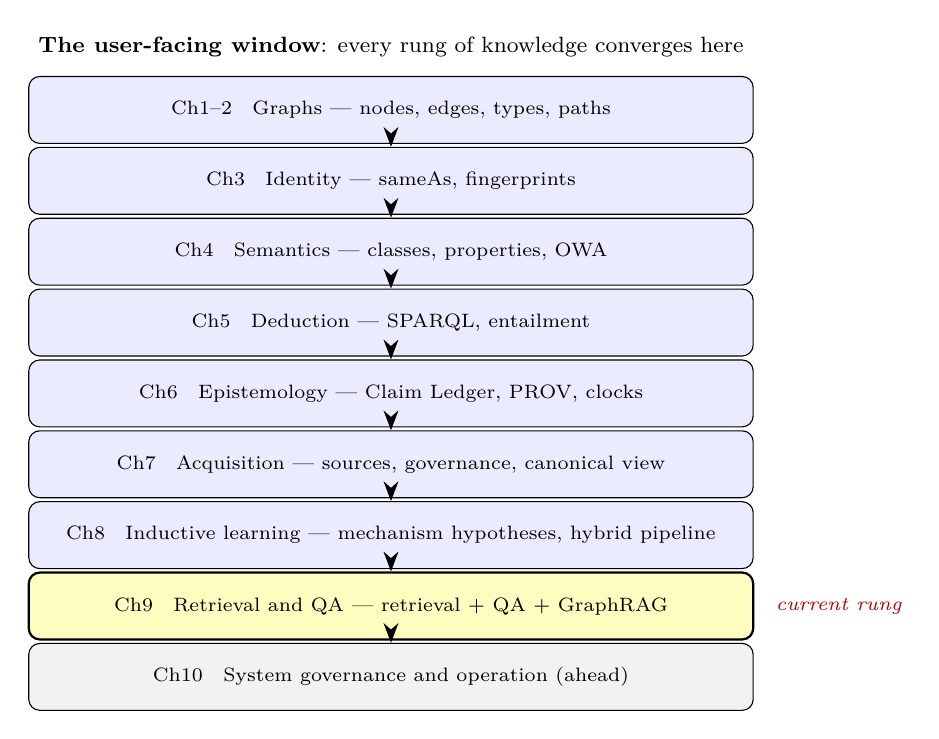
\begin{tikzpicture}[
  lvl/.style={rectangle, draw, rounded corners, minimum width=9.2cm, minimum height=0.85cm,
              font=\scriptsize, align=center},
  current/.style={lvl, fill=yellow!25, thick},
  done/.style={lvl, fill=blue!8},
  arrow/.style={-{Stealth[length=2.5mm]}, thick},
]

\node[done] (l1) at (0, 3.6) {Ch1--2 \; Graphs --- nodes, edges, types, paths};
\node[done] (l2) at (0, 2.7) {Ch3 \; Identity --- sameAs, fingerprints};
\node[done] (l3) at (0, 1.8) {Ch4 \; Semantics --- classes, properties, OWA};
\node[done] (l4) at (0, 0.9) {Ch5 \; Deduction --- SPARQL, entailment};
\node[done] (l5) at (0, 0.0) {Ch6 \; Epistemology --- Claim Ledger, PROV, clocks};
\node[done] (l6) at (0, -0.9) {Ch7 \; Acquisition --- sources, governance, canonical view};
\node[done] (l7) at (0, -1.8) {Ch8 \; Inductive learning --- mechanism hypotheses, hybrid pipeline};
\node[current] (l8) at (0, -2.7) {Ch9 \; Retrieval and QA --- retrieval + QA + GraphRAG};
\node[done, fill=gray!10] (l9) at (0, -3.6) {Ch10 \; System governance and operation (ahead)};

\draw[arrow] (l1) -- (l2);
\draw[arrow] (l2) -- (l3);
\draw[arrow] (l3) -- (l4);
\draw[arrow] (l4) -- (l5);
\draw[arrow] (l5) -- (l6);
\draw[arrow] (l6) -- (l7);
\draw[arrow] (l7) -- (l8);
\draw[arrow, dashed] (l8) -- (l9);

\node[right=0.15cm of l8.east, font=\scriptsize\itshape, text=red!70!black]
  {current rung};

\node[font=\footnotesize, align=center] at (0, 4.4)
  {\textbf{The user-facing window}: every rung of knowledge converges here};

\end{tikzpicture}
\end{document}
